\chapter*{Preface}
This 4th semester master thesis has been written a student attending the Electro-Mechanical System Design engineering line at Aalborg University. The project period spans from the 2nd of February to the 2nd of June. \newline

%\noindent The project has been made in collaboration with Aalborg Universty since the skateboard has some commercial value at different events. The project makes an analysis of the old project, which leads to some aspects a new design should improve. This includes a new improved design of the skateboard, and a more complex model of the skateboard. Lastly the project designs and implements a controller which stabilizes the skateboard, and is able to verify the model of the skateboard.\newline
\noindent The references are created based on the Harvard method, meaning that each reference is written with both author and year of publish. All figures are named X.Y, where X shows the coherent chapter and Y the figure number. Whenever a table or figure is used a describing text follows to explain the context. If the figure doesn't include a reference its made by the group itself. The chapters in the annex and appendix are written with letters to differentiate between main matter and attachments.\newline
\noindent A CD will be attached to the printed project, including the annex, appendix and all SolidWorks parts with drawings. The drawings are also printed and assembled in a separate holder, to provide easy accessibility for the reader.\newline
\textbf{Software}
The following software has been used in the process of making this project.

\begin{center}

\begin{tabular}{l l |l l}
\hline 
\textbf{Name} & \textbf{Area of use} & \textbf{Name} & \textbf{Area of use}\\ 
\hline  
\LaTeX & Assembling the project & SolidWorks & 3D drawing of the skateboard \\ 
\hline 
Maple 16 & Calculations & Ansys & FE analysis \\ 
\hline 
Matlab & Calculations and scripts & Eagle & Circuit drawing of PCB\\ 
\hline

\end{tabular} \\[2cm]

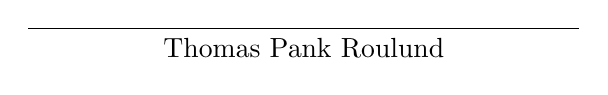
\begin{tikzpicture}[auto]
\draw (0,-1) --node[below]{Thomas Pank Roulund} (7,-1);
\end{tikzpicture}
\end{center}
